\documentclass[aspectratio=169]{beamer}

\usetheme{Madrid}
\beamertemplatenavigationsymbolsempty

%\usecolortheme{beaver}
% the following colors are modified from beaver
\definecolor{tuna}{rgb}{0.098,0.51,0.996}
\definecolor{thu}{rgb}{0.50,0.36,0.71}

\setbeamercolor{section in toc}{fg=black,bg=white}
\setbeamercolor{item}{fg=tuna,bg=white}
\setbeamercolor{alerted text}{fg=tuna!80!gray}
\setbeamercolor*{palette primary}{fg=tuna!60!black,bg=gray!30!white}
\setbeamercolor*{palette secondary}{fg=tuna!70!black,bg=gray!15!white}
\setbeamercolor*{palette tertiary}{bg=tuna!80!black,fg=gray!10!white}
\setbeamercolor*{palette quaternary}{fg=tuna,bg=gray!5!white}

\setbeamercolor*{sidebar}{fg=tuna,bg=gray!15!white}

\setbeamercolor*{palette sidebar primary}{fg=tuna!10!black}
\setbeamercolor*{palette sidebar secondary}{fg=white}
\setbeamercolor*{palette sidebar tertiary}{fg=tuna!50!black}
\setbeamercolor*{palette sidebar quaternary}{fg=gray!10!white}

%\setbeamercolor*{titlelike}{parent=palette primary}
\setbeamercolor{titlelike}{parent=palette primary,fg=tuna}
\setbeamercolor{frametitle}{bg=gray!10!white}
\setbeamercolor{frametitle right}{bg=gray!60!white}

\setbeamercolor*{separation line}{}
\setbeamercolor*{fine separation line}{}

\setbeamertemplate{sections/subsections in toc}[square]
\setbeamertemplate{items}[square]

% https://tex.stackexchange.com/questions/248131/delete-institute-space-in-title-page-beamer-class
\defbeamertemplate{title page}{noinstitute}[1][]
{
  \vbox{}
  \vfill
  \begingroup
    \centering
    \begin{beamercolorbox}[sep=8pt,center,#1]{title}
      \usebeamerfont{title}\inserttitle\par%
      \ifx\insertsubtitle\@empty%
      \else%
        \vskip0.25em%
        {\usebeamerfont{subtitle}\usebeamercolor[fg]{subtitle}\insertsubtitle\par}%
      \fi%     
    \end{beamercolorbox}%
    \vskip1em\par
    \begin{beamercolorbox}[sep=8pt,center,#1]{author}
      \usebeamerfont{author}\insertauthor
    \end{beamercolorbox}
    \begin{beamercolorbox}[sep=8pt,center,#1]{date}
      \usebeamerfont{date}\insertdate
    \end{beamercolorbox}\vskip0.5em
    {\usebeamercolor[fg]{titlegraphic}\inserttitlegraphic\par}
  \endgroup
  \vfill
}

\makeatletter
\setbeamertemplate{title page}[noinstitute][colsep=-4bp,rounded=true,shadow=\beamer@themerounded@shadow]
\makeatother

\AtBeginSection[]{
  \begin{frame}
  \vfill
  \centering
  \begin{beamercolorbox}[sep=8pt,center,shadow=true,rounded=true]{title}
    \usebeamerfont{title}\insertsectionhead\par%
  \end{beamercolorbox}
  \vfill
  \end{frame}
}

\usepackage{tikz}
\usetikzlibrary{calc}
\usetikzlibrary{arrows}
\usetikzlibrary{shapes}
\usepackage{hyperref}

\newcommand{\T}[1]{\texttt{#1}}

\title[Learn Git]{Learn Git The Not So Super Hard Way\footnote{Credit to https://github.com/b1f6c1c4/learn-git-the-super-hard-way}}
\author[zenithal]{Zenithal}
\date{2022-03-31}

\begin{document}

\begin{frame}
\titlepage
\end{frame}

\begin{frame}{Why this}
  \begin{itemize}
    \item<1-> Learning git is painful\begin{itemize}
      \item Too many concepts (commit, branch, stage, index)
      \item Too many commands (clone, pull, push)
    \end{itemize}
    \item<2-> State machine too complex\begin{itemize}
      \item You often do not know what state you are in 
      \item Conflict! Help me ERIN!
    \end{itemize}
    \item<3-> Learning about commands is not enough\begin{itemize}
      \item You often do not know what's going on
      \item Let's break it down to basic elements
    \end{itemize}
    \item<4-> The super hard way is super easy\begin{itemize}
      \item You change the file, you know what's going on
    \end{itemize}
  \end{itemize}
\end{frame}

\section{init}
\begin{frame}{git repo structure}
  \begin{itemize}
    \item git repo\begin{itemize}
      \item often the \T{.git}
      \item often contains HEAD, config
    \end{itemize}
    \item worktree\begin{itemize}
      \item the file
      \item often contains README.md, main.c, main.h
      \item worktree is just a checkout of the git repo
      \item you can re-contruct your worktree from the git repo
      \item the git repo is essential, but worktree is not
    \end{itemize}
  \end{itemize}
\end{frame}

\begin{frame}{git init}
  \begin{itemize}
    \item \T{mkdir .git}
    \item \T{mkdir .git/objects}\begin{itemize}
      \item Must have
    \end{itemize}
    \item \T{mkdir .git/refs}\begin{itemize}
      \item Must have
    \end{itemize}
    \item \T{echo 'ref: refs/heads/master' > .git/HEAD}\begin{itemize}
      \item Establish {HEAD} ref
      \item HEAD points to \T{.git/refs/heads/master} (Even though it does not exist now)
      \item Side note: \T{refs/heads/main}
    \end{itemize}
    \item config, hooks, info, etc are not necessary
    \item Now you can \T{git status} to check the status
  \end{itemize}
\end{frame}

\section{objects}
\begin{frame}{objects}
  \begin{itemize}
    \item<1-> You have created \T{.git/objects}, then what are objects
    \item<2-> Four types of objects\begin{itemize}
      \item<3-> blob: file content
      \item<4-> tree: folder\begin{itemize}
        \item Side note: what's in folder in file system
        \item filename (stored here instead of in blob!)
        \item hash of blobs/trees (folder structure!)
      \end{itemize}
      \item<5-> commit: a state of the root folder\begin{itemize}
        \item contains one specific tree
        \item parent(s): other commit(s)
        \item author/committer/commit message: meta data
      \end{itemize}
      \item<6-> tag: will not introduce today
    \end{itemize}
  \end{itemize}
\end{frame}

\begin{frame}[fragile]{blob}
  \begin{itemize}
    \item<1-> blob: file content
    \item<2-> \T{echo 'hello' | git hash-object -t blob --stdin -w}\begin{itemize}
      \item Write a blob/file whose content is \T{'hello'}
      \item hash that content to an object in type \T{blob} from \T{stdin} then \T{w}rite to the object database
      \item Output: \T{ce013625030ba8dba906f756967f9e9ca394464a}, the hash of the object
    \end{itemize}
    \item<3-> \T{cat .git/objects/ce/013625030ba8dba906f756967f9e9ca394464a}\begin{itemize}
      \item Output: \T{xKOR0cH}, compressed content of hello
      \item note the object path!
    \end{itemize}
    \item<4-> Check the actual content\begin{verbatim}
    $ printf '\x1f\x8b\x08\x00\x00\x00\x00\x00' \
    | cat - .git/objects/ce/013625030ba8dba906f756967f9e9ca394464a \
    | gunzip -dc 2>/dev/null | xxd
    # 00000000: 626c 6f62 2036 0068 656c 6c6f 0a         blob 6.hello.
    \end{verbatim}
  \end{itemize}
\end{frame}

\begin{frame}{blob (cont'd)}
  \begin{itemize}
    \item Painful using raw command? Of course we have higher level instructions
    \item \T{git cat-file blob ce01}\begin{itemize}
      \item Output: \T{hello}
    \end{itemize}
    \item \T{git show ce01}\begin{itemize}
      \item Output: \T{hello}
    \end{itemize}
  \end{itemize}
\end{frame}

\begin{frame}[fragile]{tree}
  \begin{itemize}
    \item<1-> tree: folder
    \item<2-> Create a tree\begin{verbatim}
(printf '100644 name.ext\x00';
echo '0: ce013625030ba8dba906f756967f9e9ca394464a' | xxd -rp -c 256;
printf '100755 name2.ext\x00';
echo '0: ce013625030ba8dba906f756967f9e9ca394464a' | xxd -rp -c 256) \
| git hash-object -t tree --stdin -w
# 58417991a0e30203e7e9b938f62a9a6f9ce10a9a
\end{verbatim}
    \item<3-> You can also (another format)\begin{verbatim}
git mktree --missing <<EOF
100644 blob ce013625030ba8dba906f756967f9e9ca394464a$(printf '\t')name.ext
100755 blob ce013625030ba8dba906f756967f9e9ca394464a$(printf '\t')name2.ext
EOF
# 58417991a0e30203e7e9b938f62a9a6f9ce10a9a
\end{verbatim}
  \end{itemize}
\end{frame}

\begin{frame}[fragile]{tree (cont'd)}
  \begin{itemize}
    \item<1-> Directly inspect file content\begin{verbatim}
printf '\x1f\x8b\x08\x00\x00\x00\x00\x00' \
| cat - .git/objects/58/417991a0e30203e7e9b938f62a9a6f9ce10a9a \
| gunzip -dc 2>/dev/null | xxd
\end{verbatim}
    \item<2-> \T{git cat-file tree 5841 | xxd}
    \item<3-> \T{git ls-tree 5841} (Compare with mktree above)
    \item<4-> \T{git show 5841} (A more simple version)
  \end{itemize}
\end{frame}

\begin{frame}[fragile]{commit}
  Directly create file\begin{verbatim}
git hash-object -t commit --stdin -w <<EOF
tree 58417991a0e30203e7e9b938f62a9a6f9ce10a9a
author b1f6c1c4 <b1f6c1c4@gmail.com> 1514736000 +0800
committer b1f6c1c4 <b1f6c1c4@gmail.com> 1514736000 +0800

The commit message
May have multiple
lines!
EOF
# d4dafde7cd9248ef94c0400983d51122099d312a
\end{verbatim}
\end{frame}

\begin{frame}[fragile]{commit (cont'd)}
  Or from high level command\begin{verbatim}
GIT_AUTHOR_NAME=b1f6c1c4 \
GIT_AUTHOR_EMAIL=b1f6c1c4@gmail.com \
GIT_AUTHOR_DATE='1600000000 +0800' \
GIT_COMMITTER_NAME=b1f6c1c4 \
GIT_COMMITTER_EMAIL=b1f6c1c4@gmail.com \
GIT_COMMITTER_DATE='1600000000 +0800' \
git commit-tree 5841 -p d4da <<EOF
Message may be read
from stdin
or by the option '-m'
EOF
# efd4f82f6151bd20b167794bc57c66bbf82ce7dd
\end{verbatim}
  That's why you need to \T{git config --global user.email} and \T{user.name}
\end{frame}

\begin{frame}[fragile]{commit (cont'd)}
  \begin{itemize}
    \item<1-> Directly inspect file content\begin{verbatim}
printf '\x1f\x8b\x08\x00\x00\x00\x00\x00' \
| cat - ./objects/ef/d4f82f6151bd20b167794bc57c66bbf82ce7dd \
| gunzip -dc 2>/dev/null | xxd
\end{verbatim}
    \item<2-> \T{git cat-file commit efd4}
    \item<3-> \T{git show efd4~} (A more simple version, in diff format)
    \item<3-> Note: commits are snapshots, not diffs/patchs\footnote{https://github.blog/2020-12-17-commits-are-snapshots-not-diffs/}
  \end{itemize}
\end{frame}

\begin{frame}[fragile]{Lucky commit}
  \begin{itemize}
    \item Feeling hash too boring?
    \item Try lucky commit!\footnote{https://github.com/not-an-aardvark/lucky-commit}
    \item \begin{verbatim}
$ git log
1f6383a Some commit
$ lucky_commit
$ git log
0000000 Some commit
\end{verbatim}
    \item Note the commit msg in the prev slide, we can change it to mine a lucky hash
  \end{itemize}
\end{frame}

\section{ref}
\begin{frame}{ref}
  \begin{itemize}
    \item ref is a convenient reference to one specific commit/other ref
    \item in \T{.git/ref}
    \item two types of ref\begin{itemize}
      \item direct ref
      \item indirect ref, e.g. \T{HEAD} (often the case)
    \end{itemize}
    \item two common refs we will introduce today\begin{itemize}
      \item heads: local branch
      \item remotes: remote branch
    \end{itemize}
  \end{itemize}
\end{frame}

\begin{frame}[fragile]{local branch and direct ref}
  \begin{itemize}
    \item<1-> Create file (not recommended as no reflog)\begin{verbatim}
mkdir -p .git/refs/heads/
echo d4dafde7cd9248ef94c0400983d51122099d312a > .git/refs/heads/br1
\end{verbatim}
    \item<2-> The following command will leave reflog in \T{.git/log/refs/heads/br1}
    \item<2-> \T{git update-ref --no-deref -m 'Reason for update' refs/heads/br1 d4da}
    \item<2-> \T{git branch -f br1 d4da}
  \end{itemize}
\end{frame}

\begin{frame}{about reflog}
  \begin{itemize}
    \item Record all the changes to your ref
    \item Useful when you accidently switch to another place\begin{itemize}
      \item \T{git rebase master}
      \item \T{git checkout -B master origin/master}
      \item then you want to switch to old tree for some reason
      \item reflog shows the commit that one ref \textbf{was}
    \end{itemize}
    \item Demo of my working dir: lots of reflogs
  \end{itemize}
\end{frame}

\begin{frame}{indirect ref}
  \begin{itemize}
    \item Remember when you init\begin{itemize}
      \item \T{echo 'ref: refs/heads/master' > .git/HEAD}
    \end{itemize}
    \item This format is indirect ref
  \end{itemize}
\end{frame}

\section{index}
\begin{frame}{index}
  \begin{figure}
    \centering
    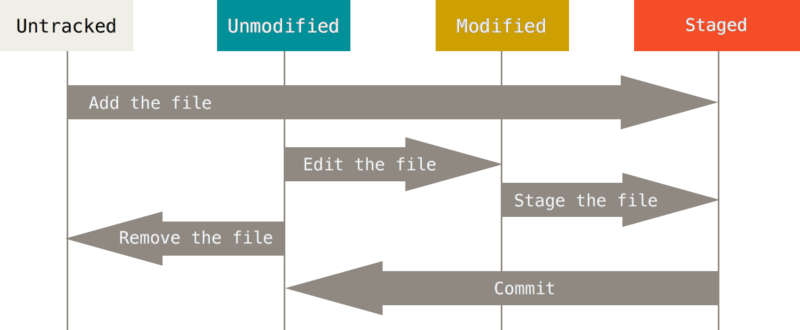
\includegraphics[width=0.7\textwidth]{img/lifecycle.png}
  \end{figure}
  \begin{itemize}
    % stage figure here
    \item index stores what to be commited when you \T{git commit}
    \item file at \T{.git/index}
    \item often we call things in index as staged (the figure above)
    \item a complex database
    \item contains many things, like filename, mode, hash, mtime, etc
  \end{itemize}
\end{frame}

\begin{frame}{manipulate index}
  \begin{itemize}
    \item<1-> it is hard to manupulate index  
    \item<1-> we study common cases here
    \item<1-> \T{git add} stores the content into index
    \item<1-> mark them ready for commit
    \item<2-> 1. \T{git add; git status}\begin{itemize}
      \item the file you added is ready for commit
    \end{itemize}
    \item<3-> 2. \T{git add; modify; git status}\begin{itemize}
      \item the file content you added is ready for commit
      \item the new file content you did not add is not visible to index
      \item \T{modify} will not be contained in commit
    \end{itemize}
    \item<4-> 3. \T{git add; rm; git status; git restore}\begin{itemize}
      \item even though file is deleted, it has a copy in \T{index}
      \item if you accidently \T{rm -rf *}, you can restore your file! 
    \end{itemize}
  \end{itemize}
\end{frame}

\section{switch/checkout}
\begin{frame}{switch/checkout}
  \begin{itemize}
    \item Recall that \T{.git/HEAD} is a ref
    \item This ref is for your worktree
    \item Recall your worktree is your actual content
    \item Change the content of your worktree by manipulating HEAD
  \end{itemize}
\end{frame}

\begin{frame}{switch/checkout (cont'd)}
  \begin{itemize}
    \item<1-> Most famous: \T{git checkout master}\begin{itemize}
      \item Make HEAD point to \T{refs/heads/master}
      \item Then checkout the content to your worktree
      \item That's why it is named checkout
      \item Actually an old syntax, recommend using switch now
      \item \T{git switch master}
    \end{itemize}
    \item<2-> Yet most famous: \T{git reset --hard HEAD$\sim$1}\begin{itemize}
      \item Change HEAD to HEAD$\sim$1 (the former commit of HEAD)
      \item Checkout the content to your worktree
      \item Note: there are \T{reset --soft/--mixed}, learn them by yourself
    \end{itemize}
  \end{itemize}
\end{frame}

\section{pull/clone/push}
\begin{frame}{remotes}
  \begin{itemize}
    \item Recall that we have talked about \T{.git/refs/remotes}
    \item Since we have local ref(branch), we can also have remote ref(branch)
    \item If no remote branch, it is not a distributed version control system
    \item How to sync them?
    \item pull commit from remote to local
    \item push commit from local to remote
    \item So the concept of commit is very useful
  \end{itemize}
\end{frame}

\begin{frame}{config remote}
  \begin{itemize}
    \item If you want to have remote branch, you must have a remote first
    \item edit \T{.git/config} to add them
    \item or \T{git remote add origin git@github.com:xxx/yyy}\begin{itemize}
      \item \T{origin} is a convention, you can use other name
      \item You can have multiple remote
    \end{itemize}
    \item Demo of my repo
  \end{itemize}
\end{frame}

\begin{frame}{fetch remote}
  \begin{itemize}
    \item<1-> \T{git fetch origin master}\begin{itemize}
      \item Fetch the \T{master} ref from \T{origin}
      \item You can check \T{.git/refs/remotes/origin/master} now
    \end{itemize}
    \item<2-> \T{git pull origin master}\begin{itemize}
      \item despite \T{git fetch}, it tries to update your local ref
      \item Update \T{.git/refs/remotes/origin/master}
      \item and update \T{.git/refs/heads/master} accordingly
      \item The relationship is recorded in \T{.git/config}
    \end{itemize}
    \item<3-> \T{git pull}\begin{itemize}
      \item short hand for the above, according to your \T{.git/config}
    \end{itemize}
    \item<4-> \T{git clone}\begin{itemize}
      \item Actually a short hand for
      \item \T{git init}
      \item \T{git remote add}
      \item \T{git pull}
    \end{itemize}
  \end{itemize}
\end{frame}

\begin{frame}{push remote}
  \begin{itemize}
    \item<1-> \T{git push origin master}\begin{itemize}
      \item Sync your local branch master to remote branch master
    \end{itemize}
    \item<2-> \T{git push}\begin{itemize}
      \item short hand for the above, according to your \T{.git/config}
    \end{itemize}
    \item<3-> New branch then \T{git push -u origin :new-branch}\begin{itemize}
      \item Add a new ref in the remote
      \item At the same time set the upstream to new-branch
      \item Check your \T{.git/config} now
    \end{itemize}
  \end{itemize}
\end{frame}

\section{merge}
\begin{frame}{merge}
  \begin{itemize}
    \item Now you have commits, you have refs
    \item How do you merge refs/branches together?
    \item recall that a branch points to a commit, a commit contains a specific tree
    \item Namely we need to merge tree, then we need to merge blob first
    \item How to merge blob?
  \end{itemize}
\end{frame}

\begin{frame}{two way merge}
  \begin{itemize}
    \item Two way means the algo can only see two files (our and their)
    \item Let's setup the file as \T{chapter6.md}
    \item Two way merge of \T{fileB} and \T{fileC}\begin{itemize}
      \item The change can be fileC has removed B in the first line and added C in the last line
      \item The change can be fileB has added B in the first line and deleted C in the last line
      \item Do not know how to merge, abort
    \end{itemize}
    \item It is not useful
  \end{itemize}
\end{frame}

\begin{frame}[fragile]{three way merge}
  \begin{itemize}
    \item Three way merge means the algo can see three files (base, our and their)
    \item Three way merge of \T{fileB} and \T{fileC} with \T{fileA} as base\begin{itemize}
      \item Compared with \T{fileA}, \T{fileB} added B in the first line
      \item Compared with \T{fileA}, \T{fileC} added C in the last line
      \item No conflict in changes
      \item \T{git merge-file --stdout <our> <base> <their>}
      \item \T{git merge-file --stdout fileC fileA fileB}\begin{verbatim}
lineBB
...some stuff...
lineCC
\end{verbatim}
    \end{itemize}
  \end{itemize}
\end{frame}

\begin{frame}[fragile]{three way merge (cont'd)}
  \begin{itemize}
    \item What if they both modify the same line? Conflict!
    \item Usually need manual involvement
    \item E.g. \T{git merge-file --stdout fileD fileA fileB}\begin{itemize}
      \item Compared with \T{fileA}, \T{fileD} added D in the first line
      \item Compared with \T{fileA}, \T{fileB} added B in the first line
      \item Output\begin{verbatim}
<<<<<<< fileD
lineBD
=======
lineBB
>>>>>>> fileB
...some stuff...
lineC
\end{verbatim}
    \end{itemize}
  \end{itemize}
\end{frame}

\begin{frame}[fragile]{How to resolve conflict}
  \begin{itemize}
    \item Remove all the helper line
    \item Leave the actual content\begin{verbatim}
lineBBD
...some stuff...
lineC
\end{verbatim}
    \item Or if you are aware of what you are doing\begin{itemize}
      \item \T{git merge-file --ours --stdout fileD fileA fileB}
      \item Keep our change, discard theirs
      \item \T{git merge-file --theirs --stdout fileD fileA fileB}
      \item Keep their change, discard ours
      \item \T{git merge-file --union --stdout fileD fileA fileB}
      \item Keep both changes, concat them
    \end{itemize}
  \end{itemize}
\end{frame}

\end{document}

% vim: nospell
